\chapter{Smart Home Viewer}
Smart Home Viewer est une application de télémaintenance permettant de faire le diagnostique de la connexion internet d'un modem internet.
\begin{figure}[H]
	\centering
	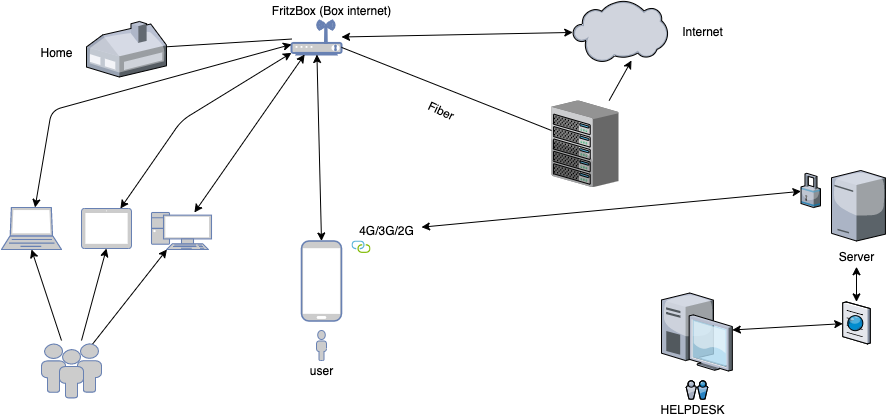
\includegraphics[scale=0.4]{assets/images/shv.png}
	\caption{Description global du système de fonctionnement de l'application}
	\label{fig.3}
\end{figure} 
Le contexte de fonctionnement de l'application est lorsque pour une raison ou une autre, un utilisateur de la box de l'entreprise voit sa connexion internet s'interrompre. Dans ce cas, il appelle le centre d'appel de l'entreprise et l'operateur lui fournit un code de connexion pour le diagnostique de sa connexion.

Le processus de diagnostique de la connexion est décrit sur la figure \ref{fig.3}. Pour faire fonctionner l'application, l'utilisateur devra activer son Wifi et ses données mobiles. La liaison Wifi servira à la communication avec la box et les données mobiles serviront à envoyer les données de la box au serveur.

Lorsque l'utilisateur s'authentifie avec le code que l'opérateur lui a fourni, l'opérateur, le téléphone est prêt pour servir de canal de transmission de l'information entre la box et le serveur. L'opérateur déclenche la communication entre les appareils puis le serveur envoie les requêtes nécessaires à la box pour récupérer et afficher la page d'accueil de la box directement sur le poste de l'opérateur qui pourra vérifier les paramètres et faire des modifications si nécessaire.

Dans la suite, il sera décrit le fonctionnement du système.
\section{Contexte du système}
Dans cette section je présente le diagramme de contexte du système afin de localiser l'application dans son environnement. Il est aussi décrit les acteurs qui interagissent avec le système. Dans la suite de ce chapitre, \textit{Modem} fait référence à la box.
\begin{figure}[H]
	\centering
	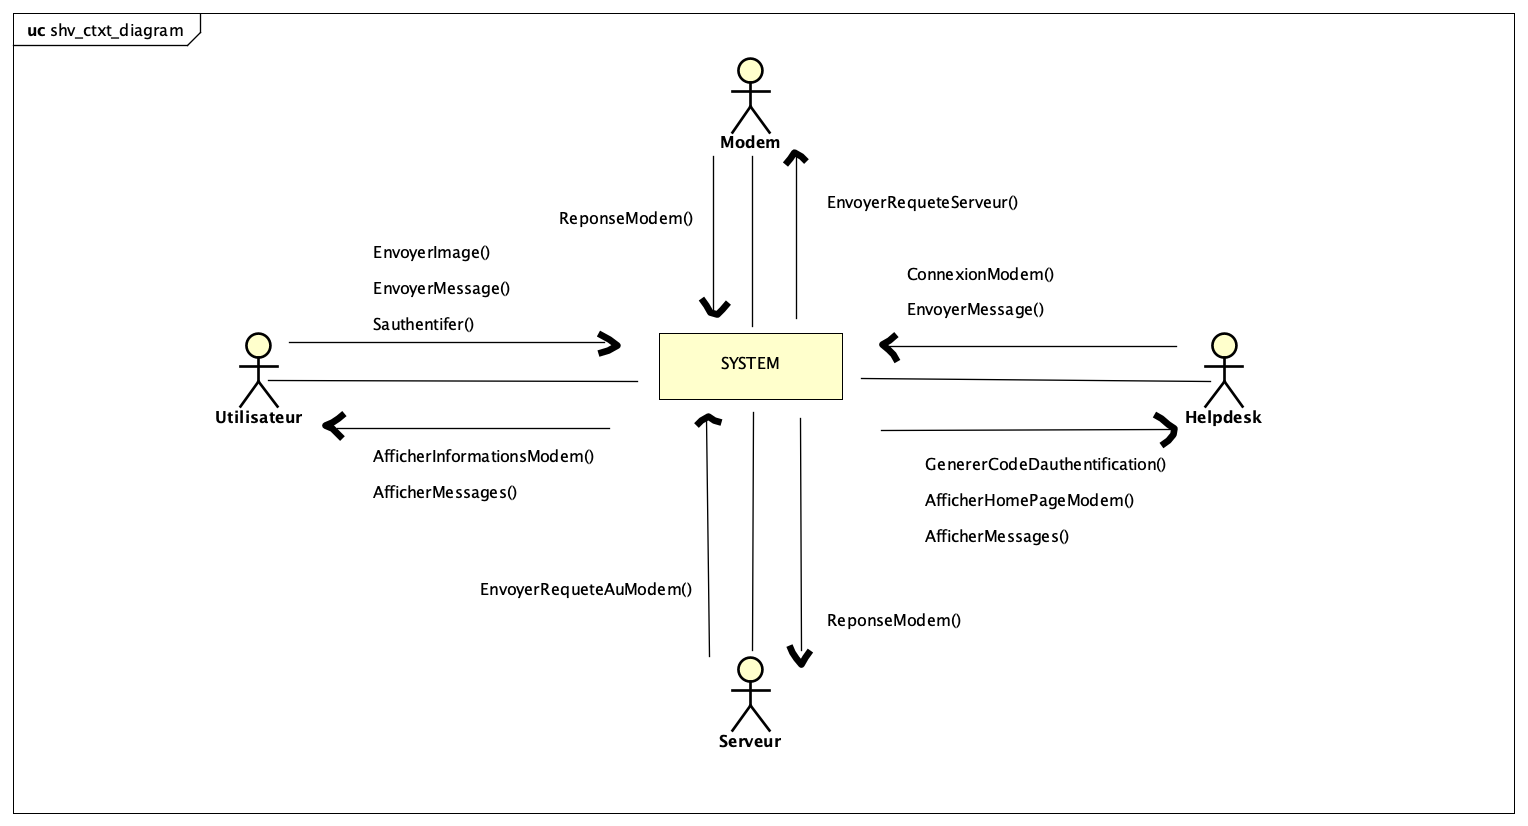
\includegraphics[scale=0.4]{assets/images/shv_ctxt.png}
	\caption{Diagramme de contexte}
	\label{fig.3}
\end{figure} 

\emph{L'utilisateur} et le \hd sont les acteurs principaux du système. Afin d'initier la communication, le \hd doit fournir le code d'authentification à l'utilisateur. Le code d'authentification est généré par le système côté serveur et fourni au \hd. \textit{GenererCodeDauthentification()} consiste à générer un code à six chiffres, l'associer à une session et à l'afficher au \hd. L'\emph{utilisateur} se connecte au système via ce code. Il réalise cette connexion via \textit{Sauthentifier()}. Une fois authentifier, le système côté client effectue quelques requêtes afin d'afficher à l'utilisateur, les informations de son Modem. Les informations sont affichées via \textit{AfficherInformationsModem()}. Le \hd et l'\emph{utilisateur} peuvent s'échanger via un chat et les fonctions principales de ce chat est l'envoie des messages et d'images. Ces fonctions sont réalisées via \textit{EnvoyerMessage()}, \textit{EnvoyerImage()} et \textit{AfficherMessages()}.

 Une fois la connexion réalisée par l'\emph{utilisateur}, le \hd, peut déclencher l'affichage de la page d'accueil du modem. Si la requête est fait, le serveur envoie et reçoit des requêtes au système via les fonctions \textit{EnvoyerRequeteAuModem()} et \textit{ReponseModem()}. Le système récupère la requête du serveur, construit une nouvelle requête spécifique et l'envoie au modem qui répond au système en retour en fonction des éléments demandés. Les fonctions misent à contributions sont \textit{EnvoyerRequeteServeur()} et \textit{ReponseModem()}. Si tout se passe bien, le serveur construit à partir des éléments fournis par le modem la page d'accueil du modem et l'affiche au \hd.
 
Du point de vue du fonctionnement du système, les acteurs \emph{Modem} et \emph{Serveur} sont certes secondaires mais indispensable. C'est la connexion internet du modem qui est diagnostiquée. Le serveur a pour rôle de servir d'interface pour le \hd et de serveur pour l'application du point de vue de l'architecture client-serveur pour une application. Le système sert donc d'intermédiaire ou de moyen de communication entre le \emph{modem} et le \emph{serveur}.

\section{Caractéristique de l'utilisateur}
L'application est destinée à l'utilisation des clients de la société \lol ayant souscris à une offre internet via box ou ADSL. L'utilisation de l'application ne requiert aucune compétence particulière à part le fait de savoir utiliser un smartphone.

\section{Contraintes principaux de développements}
L'application a été développé pour les deux plateformes mobiles Android et iOS et selon le paradigme orienté objet. Pour ce faire j'ai utilisé le langage de programmation Java\footnote{Java est un langage de programmation objet créé par Sun microsystems et détenu depuis 2009 par Oracle. }, l'environnement de  développement d'application Android et l'IDE Android Studio pour l'application Android et le les langages Swift\footnote{Swift est un langage de programmation objet, multiparadigme, open-source développé par Apple en 2014 } et Objective C\footnote{Objective C est un langage orienté objet réflexif créé en 1983 et détenu par Apple.} avec l'environnement de développement d'application Cocoa Touch et l'IDE XCode pour l'application iOS. 

J'ai aussi utilisé des standards RFC pour des questions réseaux.

\section{Besoins fonctionnels}
